%% Creator: Inkscape inkscape 0.91, www.inkscape.org
%% PDF/EPS/PS + LaTeX output extension by Johan Engelen, 2010
%% Accompanies image file 'funnel.pdf' (pdf, eps, ps)
%%
%% To include the image in your LaTeX document, write
%%   \input{<filename>.pdf_tex}
%%  instead of
%%   \includegraphics{<filename>.pdf}
%% To scale the image, write
%%   \def\svgwidth{<desired width>}
%%   \input{<filename>.pdf_tex}
%%  instead of
%%   \includegraphics[width=<desired width>]{<filename>.pdf}
%%
%% Images with a different path to the parent latex file can
%% be accessed with the `import' package (which may need to be
%% installed) using
%%   \usepackage{import}
%% in the preamble, and then including the image with
%%   \import{<path to file>}{<filename>.pdf_tex}
%% Alternatively, one can specify
%%   \graphicspath{{<path to file>/}}
%% 
%% For more information, please see info/svg-inkscape on CTAN:
%%   http://tug.ctan.org/tex-archive/info/svg-inkscape
%%
\begingroup%
  \makeatletter%
  \providecommand\color[2][]{%
    \errmessage{(Inkscape) Color is used for the text in Inkscape, but the package 'color.sty' is not loaded}%
    \renewcommand\color[2][]{}%
  }%
  \providecommand\transparent[1]{%
    \errmessage{(Inkscape) Transparency is used (non-zero) for the text in Inkscape, but the package 'transparent.sty' is not loaded}%
    \renewcommand\transparent[1]{}%
  }%
  \providecommand\rotatebox[2]{#2}%
  \ifx\svgwidth\undefined%
    \setlength{\unitlength}{352.09962845bp}%
    \ifx\svgscale\undefined%
      \relax%
    \else%
      \setlength{\unitlength}{\unitlength * \real{\svgscale}}%
    \fi%
  \else%
    \setlength{\unitlength}{\svgwidth}%
  \fi%
  \global\let\svgwidth\undefined%
  \global\let\svgscale\undefined%
  \makeatother%
  \begin{picture}(1,1.43141304)%
    \put(0,0){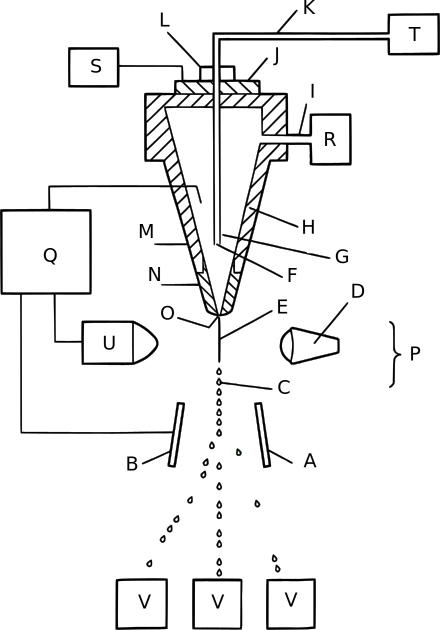
\includegraphics[width=\unitlength,page=1]{nozzle.pdf}}%
    \put(0.6896202,0.36966639){\color[rgb]{0,0,0}\makebox(0,0)[lb]{\smash{\alab{n:A}}}}%
    \put(0.2852193,0.36252993){\color[rgb]{0,0,0}\makebox(0,0)[lb]{\smash{\alabdup{n:A}}}}%
    \put(0.63014946,0.53618448){\color[rgb]{0,0,0}\makebox(0,0)[lb]{\smash{\alab{n:C}}}}%
    \put(0.79666748,0.75503664){\color[rgb]{0,0,0}\makebox(0,0)[lb]{\smash{\alab{n:D}}}}%
    \put(0.62777066,0.71935421){\color[rgb]{0,0,0}\makebox(0,0)[lb]{\smash{\alab{n:E}}}}%
    \put(0.65155897,0.79071907){\color[rgb]{0,0,0}\makebox(0,0)[lb]{\smash{\alab{n:F}}}}%
    \put(0.76098505,0.83353809){\color[rgb]{0,0,0}\makebox(0,0)[lb]{\smash{\alab{n:G}}}}%
    \put(0.68486253,0.90014522){\color[rgb]{0,0,0}\makebox(0,0)[lb]{\smash{\alab{n:H}}}}%
    \put(0.70389318,1.209393){\color[rgb]{0,0,0}\makebox(0,0)[lb]{\smash{\alab{n:I}}}}%
    \put(0.623013,1.29265198){\color[rgb]{0,0,0}\makebox(0,0)[lb]{\smash{\alab{n:J}}}}%
    \put(0.6872414,1.39969933){\color[rgb]{0,0,0}\makebox(0,0)[lb]{\smash{\alab{n:K}}}}%
    \put(0.36134182,1.37115336){\color[rgb]{0,0,0}\makebox(0,0)[lb]{\smash{\alab{n:L}}}}%
    \put(0.31376524,0.89062989){\color[rgb]{0,0,0}\makebox(0,0)[lb]{\smash{\alab{n:M}}}}%
    \put(0.33517468,0.79309793){\color[rgb]{0,0,0}\makebox(0,0)[lb]{\smash{\alab{n:N}}}}%
    \put(0.36372065,0.7050813){\color[rgb]{0,0,0}\makebox(0,0)[lb]{\smash{\alab{n:O}}}}%
    \put(0.929882,0.61230693){\color[rgb]{0,0,0}\makebox(0,0)[lb]{\smash{\alab{n:P}}}}%
    \put(0.09729177,0.83591682){\color[rgb]{0,0,0}\makebox(0,0)[lb]{\smash{\flab{n:Q}}}}%
    \put(0.73481795,1.09996687){\color[rgb]{0,0,0}\makebox(0,0)[lb]{\smash{\flab{n:R}}}}%
    \put(0.20433907,1.26648487){\color[rgb]{0,0,0}\makebox(0,0)[lb]{\smash{\flab{n:S}}}}%
    \put(0.93226073,1.34260746){\color[rgb]{0,0,0}\makebox(0,0)[lb]{\smash{\flab{n:T}}}}%
    \put(0.23764267,0.6408529){\color[rgb]{0,0,0}\makebox(0,0)[lb]{\smash{\flab{n:U}}}}%
    \put(0.31376524,0.04852434){\color[rgb]{0,0,0}\makebox(0,0)[lb]{\smash{\flab{n:V}}}}%
    \put(0.48028326,0.04852434){\color[rgb]{0,0,0}\makebox(0,0)[lb]{\smash{\flabdup{n:V}}}}%
    \put(0.64680124,0.05328207){\color[rgb]{0,0,0}\makebox(0,0)[lb]{\smash{\flabdup{n:V}}}}%
  \end{picture}%
\endgroup%
